\section{Einleitung und Motivation}
\label{sec:EinleitungundMotivation}

Der Zeeman-Effekt wird als Aufspaltung der Energieniveaus von Atomen unter dem Einfluss eines äußeren Magnetfeldes beschrieben, was dann zu einer Aufspaltung und Polarisation der Spektrallinien führt. Das Ziel des durchgeführten Versuchs ist der Effekt mithilfe einer Cadmium-Lampe nachgewiesen zu werden beziehungsweise die Aufspaltung der Spektrallinien sichtbar zu machen.

\section{Theorie}
\label{sec:Theorie}

\subsection{Das magnetische Moment eines Elektrons und seine Drehimpulse}
\label{sec:DasmagMoment}
In einem Atom besitzen die Hüllenelektronen einen Bahndrehimpuls $\vec{l}$ und einen Spin $\vec{s}$, also zwei Drehimpulse, deren Beträge sich aus den Quantenzahlen $l$ und $s$ wie folgt ergeben:
\begin{align}
|\vec{l}|&=\sqrt{l(l+1)}\hbar,\\
|\vec{s}|&=\sqrt{s(s+1)}\hbar.
\end{align}
wobei der Spin des Elektrons den Wert $s = \frac{1}{2}$ besitzt und die Bahndrehimpulsquantenzahl $l$, die in Abhängigkeit von der Hauptquantenzahl $n$ von $0$ bis $n-1$ laufen kann. 

Mit der Ladung des Elektrons können den Drehimpulsen ein magnetisches Moment zugeordnet werden, welches proportional zum sogenannten Bohrschen Magneton $\mu_\text{B}$ ist:
\begin{equation}
\mu_{\text{B}} = -\frac{1}{2} e_0 \frac{\hbar}{m_0},
\end{equation}
wobei $e_0$ die Elektronenladung und $m_0$ die Elektronenmasse sind. Die zu den Drehimpulse gehörende magnetischen Momente ergeben sich wie folgt:
\begin{align}
\vec{\mu}_l=-\frac{\mu_\text{B}}{\hbar}\vec{l}&=-\mu_\text{B}\sqrt{l(l+1)}\,\vec{l}_\text{e},\\
\vec{\mu}_s=-g_s\frac{\mu_\text{B}}{\hbar}\vec{s}&=-g_s\mu_\text{B}\sqrt{s(s+1)}\,\vec{s}_\text{e},
\end{align}
mit den Einheitsvektoren $\vec{s}_\text{e}$ und $\vec{l}_\text{e}$ in $\vec{s}-$ und $\vec{l}-$ Richtung. Die neu hinzugefügte Größe $g_s$ wird als Landé-Faktor bezeichnet und beschreibt auch die magnetomechanische Anomalie des Elektrons, also folgend aus der Dirac-Theorie besitzt dieser Faktor den Wert $2$.

\subsection{Wechselwirkungsarten der Drehimpulse}
\label{sec:Wechselwirkungen}
Die Spins und die Bahndrehimpulse können im Allgemeinen auf verschiedenste Arten miteinander wechselwirken. In der Natur werden allerdings nur zwei Grenzfälle näher betrachtet. Außerdem spielen noch die Drehimpulse des Atomkerns eine wichtige Rolle.

\subsubsection{j-j-Kopplung}
Für diesen Grenzfall werden nur die schwersten Atome betrachtet, also Atome mit einer höheren Ordnungszahl. Diese Wechselwirkung wird dadurch kennzeichnet, dass sie stärker zwischen Spin und Bahndrehimpuls des einzelnen Elektrons ist als die Wechselwirkung zwischen den verschiedenen Elektronen untereinander. Es ergibt also für jedes Einzelelektron ein Gesamtdrehimpuls von:
\begin{align}
\vec{j}_i=\vec{l}_i+\vec{s}_i
\end{align}
und ein Gesamtdrehimpuls der Hülle:
\begin{align}
\vec{J}=\sum\vec{j}_i.
\end{align}
Allerdings spielt dieser Grenzfall für den Versuch keine Rolle.

\subsubsection{LS-Kopplung}
Bei den Atomen niedriger Ordnungszahl finden die Wechselwirkungen zwischen den verschiedenen Hüllenelektronen statt. Es werden die einzelnen Bahndrehimpulse $\vec{l}$ und Spins $\vec{s}$ zu einem Gesamtdrehimpuls $\vec{L}$ und Gesamtspin $\vec{S}$ addiert:
\begin{align}
\vec{L}&=\sum\vec{l}_i, & \text{mit }|\vec{L}|=\sqrt{L(L+1)}\hbar,\\
\vec{S}&=\sum\vec{s}_i, & \text{mit }|\vec{S}|=\sqrt{S(S+1)}\hbar,
\end{align}
wobei die Quantenzahl $L$ ganzzahlig ist, während $S$ auch halbzahlige Werte annehmen kann. Für die magnetischen Momente folgt damit:
\begin{align}
|\vec{\mu}_L|&=\mu_\text{B}\sqrt{L(L+1)},\\
|\vec{\mu}_S|&=g_S\mu_\text{B}\sqrt{S(S+1)},
\end{align}
wobei hier wieder die Anomalie berücksichtigt werden muss.
Ohne den Einfluss starker Magnetfelder addieren sich $\vec{L}$ und $\vec{S}$ zum Gesamtdrehimpuls der Elektronenhülle:
\begin{align}
\vec{J}&=\vec{L}+\vec{S}, & \text{mit }|\vec{J}|=\sqrt{J(J+1)}\hbar, \\
\end{align}
was als LS- oder Russel-Saunders-Kopplung bezeichnet wird. Die entsprechende Quantenzahl $J$ ist ganz- oder halbzahlig, je nachdem ob $S$ ganz- oder halbzahlig ist.

\subsection{Aufspaltung der Energieniveaus im Magnetfeld}
Um das magnetische Moment der zugehörenden Gesamtdrehimpulses $\vec{J}$ zu bestimmen, werden zuerst die magnetische Momente des Gesamtspins $\vec{S} $ und des Gesamtbahndrehimpulses $\vec{L}$ wie folgt zusammengesetzt:
\begin{align}
\vec{\mu}_J=\vec{\mu}_L+\vec{\mu}_S.
\end{align} 
wobei hier ein Problem auftritt. Da die Richtungen von $\vec{\mu}$ und $\vec{J}$ nicht zusammenfallen, verschwindet mithilfe von der Quantenmechanik die zu den Gesamtdrehimpuls $\vec{J}$ gehörende senkrechte $\mu$-Komponente. Also es bleibt nur noch eine zu $\mu$ parallele Komponente übrig und unter andere Betrachtungen gilt für den Betrag:
\begin{align}
|\vec{\mu}_J|=g_J\mu_\text{B}\sqrt{J(J+1)}
\end{align}
mit dem Landé-Faktor:
\begin{align}
g_J=\frac{3J(J+1)+S(S+1)-L(L+1)}{2J(J+1)}. \label{eqn:lande}
\end{align}
Die Richtungsquantelung besagt nun, dass unter Einfluss eines äußeren Magnetfelds $\vec{B}$ die Winkel zwischen $\vec{\mu}$ und $\vec{B}$ so zu beschaffen sind, dass die Komponente $\mu_{J_z}$ ein ganzzahliges Vielfaches des Bohrschen Magnetons ist:
\begin{align}
\mu_{J_z}=-mg_J\mu_\text{B}, &&\text{mit } m=-J,\,-J+1,\,...,\,J-1,\,J.
\end{align}
wobei $m$ die Orientierungsquantenzahl ist, die ganzzahlige Werte annehmen kann. Ein magnetisches Moment erhält im äußeren Feld also die zusätzliche Energie: 
\begin{align}
E_\text{mag}=-\vec{\mu}_J\cdot\vec{B}=mg_J\mu_\text{B}B,
\label{eqn:emag}
\end{align}
also es sind jetzt Aufspaltungen des Energieniveaus in $2J+1$ äquidistante Niveaus möglich. Diese sind in der Abbildung \ref{fig:aufspaltungbeispiel} zu sehen. Da auch bei den angeregten Niveaus im Magnetfeld die Aufspaltung auftreten kann, sind zusätzliche Übergänge zwischen den neuen Energieniveaus möglich, was sich in einer Aufspaltung der Spektrallinien äußert. Diese Erscheinung wird als Zeeman-Effekt bezeichnet.
\begin{figure}[h!]
	\centering
	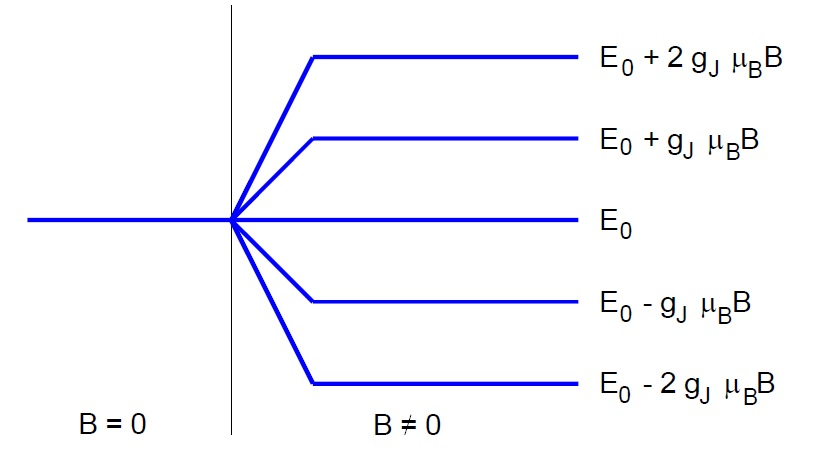
\includegraphics[width=0.7\linewidth]{content/AufspaltungBeispiel}
	\caption{Aufspaltung eines Energieniveaus mit $J = 2$, \cite[5]{anleitungV27}.}
	\label{fig:aufspaltungbeispiel}
\end{figure}

\subsection{Auswahlregeln}
Durch Lösen der zeitabhängigen Schrödinger-Gleichung sind die Übergänge in der Elektronenhülle nur zwischen Zuständen möglich, bei denen sich die Orientierungsquantenzahl $m$ gar nicht oder um $\Delta m = \pm 1$ ändert. Ist $\Delta m = 0$ entspricht dies einer Dipolschwingung parallel zum Magnetfeld, es wird linear polarisiertes Licht parallel zu $\vec{B}$ emittiert. Die Übergänge mit $\Delta m = \pm 1$ emittieren zirkulär um die Magnetfeldachse polarisiertes Licht.

\subsection{Der normale Zeeman-Effekt}
Es wird von dem normalen Zeeman-Effekt gesprochen, wenn der Gesamtspin der Elektronenhülle verschwindet, also $S = 0$. Der Landé-Faktor ist für spinlose Zustände immer $g_J = 1$ und es ergibt sich für die Verschiebung der Energieniveaus nach Gleichung \ref{eqn:emag} unabhängig von den Quantenzahlen $L$ und $J$:
\begin{align}
\Delta E=m\mu_\text{B}B.
\end{align}
Es ergibt sich also eine äquidistante Aufspaltung der Energieniveaus in $2J+1$ Unterniveaus, wie auch in Abbildung \ref{fig:normalerzeemaneffekt} zu sehen ist.
\begin{figure}[h!]
	\centering
	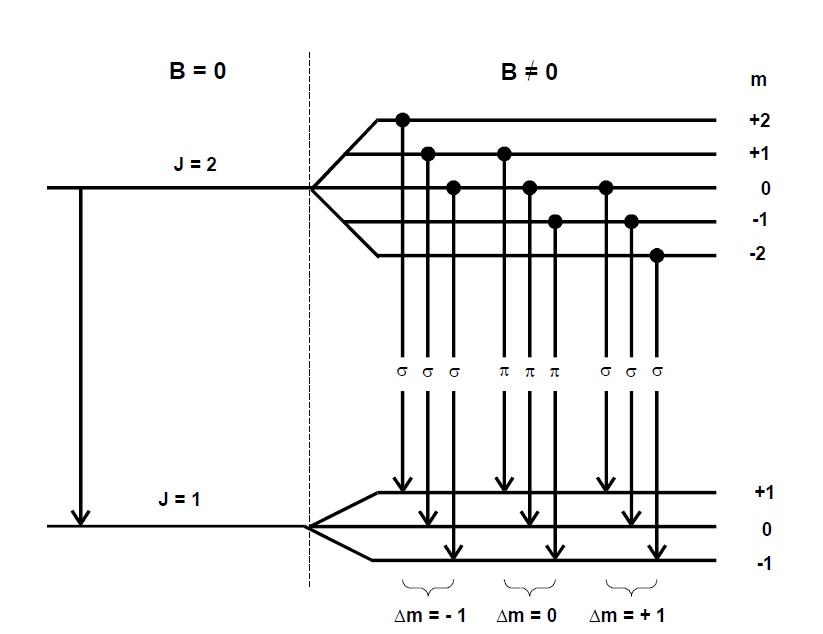
\includegraphics[width=0.7\linewidth]{content/NormalerZeemanEffekt}
	\caption{Der normale Zeeman-Effekt, \cite[10]{anleitungV27}.}
	\label{fig:normalerzeemaneffekt}
\end{figure}
Hierbei werden anhand der Polarisation die Linien kategorisiert und zwar die $\sigma_-$-Linie mit zirkularer Polarisation um das Magnetfeld bei $\Delta m = -1$, $\sigma_+$-Linie mit zirkularer Polarisation um das Magnetfeld bei $\Delta m = +1$ und $\pi$-Linie mit linearer Polarisation um das Magnetfeld bei $\Delta m = 0$. Die Energiedifferenzen verschiedener Übergänge sind gleich, wenn die entsprechenden $\Delta m$ gleich sind. Dies führt dazu, dass immer eine Aufspaltung in drei Spektrallinien beobachtet(vgl. \ref{fig:normalerzeemaneffekt}).
Aufgrund der Polarisation können nicht die Linien aus jeder Richtung gesehen werden. Die $\pi$-Linie ist aus Feldrichtung bzw. aus longitudinaler Beobachtungsrichtung nicht zu sehen, mit maximaler Intensität dazu. Werden die $\sigma$-Linien senkrecht zur Feldrichtung beobachtet, erscheinen sie ebenfalls linear polarisiert, jedoch senkrecht zur Polarisationsrichtung der $\pi$-Linie. Das Aufspaltungsbild dazu sieht wie folgt aus:
\begin{figure}[h!]
	\centering
	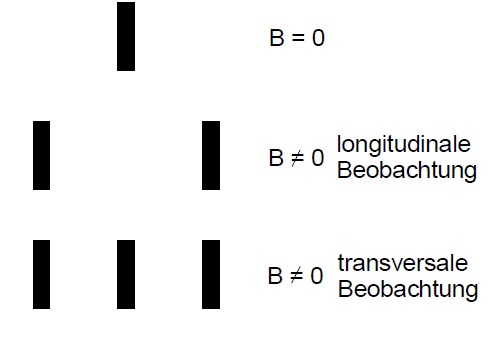
\includegraphics[width=0.7\linewidth]{content/Aufspaltungsbild}
	\caption{Aufspaltungsbild beim normalen Zeeman-Effekt, \cite[10]{anleitungV27}.}
	\label{fig:aufspaltungsbild}
\end{figure}
\subsection{Der anormale Zeeman-Effekt}
Anders als bei dem normalen Zeeman-Effekt werden beim anormalen Zeeman-Effekt nur Zustände beobachtet, die einen Spin enthalten also einen Gesamtspin in der Elektronenhülle. Die gleichen Auswahlregeln gelten ebenfalls auch für den anormalen Zeeman-Effekt. Der Unterschied zum normalen Zeeman-Effekt besteht darin, dass die Energiedifferenzen vom Spin abhängig sind, weil $g_J$ nicht mehr den Wert $1$ annimmt sondern verschiedene. Die Energieverschiebung ist in diesem Fall gegeben wie folgt:
\begin{align}
E=(m_1g(L_1,S_1,J_1)-m_1g(L_1,S_1,J_1))\mu_\text{B}B+E_0, \label{eqn:Eanomal}
\end{align}
wobei $E_0$ die Energie bei $B=0$ ist und die Indizes die Zugehörigkeit zu den zwei verschiedenen Übergangsniveaus angeben sollen. Ein Beispiel zu dem normalen Zeeman-Effekt wird in der Abbildung \ref{fig:anormalerzeemaneffekt} illustriert. Beim anormalen ist die Aufspaltung deutlich linienreicher.
\begin{figure}[h!]
	\centering
	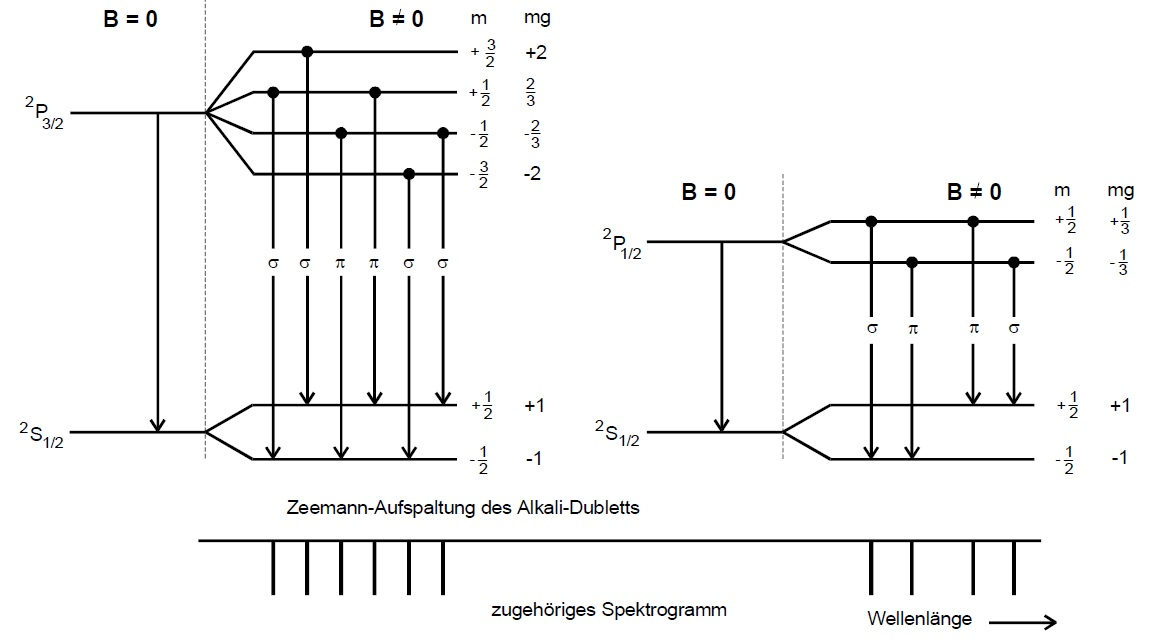
\includegraphics[width=0.9\linewidth]{content/AnormalerZeemanEffekt}
	\caption{Der anormale Zeeman-Effekt, \cite[11]{anleitungV27}.}
	\label{fig:anormalerzeemaneffekt}
\end{figure}
